\section{System Identification \label{sec::sysID}}

The switched model~(\ref{eqn::switched_model}) has two parameter vectors: $\theta_{\sat}$ (saturation
ceiling,~\ref{eqn::eta_sat}) and $\theta_{\nox}$ (unsaturated dynamics and guard
condition,~\ref{eqn::eta_bar_dynamics},~\ref{eqn::guard_condition}). The goal is to estimate both from available
measurement data ($u_1, x_1, u_2, F, T$). The guard condition $G(k) = \phi_g^T(k)\,\theta_{\nox}$ depends on
$\theta_{\nox}$, so the operating mode is not known a priori. We address this by first estimating $\theta_{\sat}$ via
linear programming (mode-independent), then using the estimated saturation ceiling to identify data segments near
saturation, and finally estimating $\theta_{\nox}$ from the remaining unsaturated data.

% ===========================================================
\subsection{Saturated Model Parameters ($\theta_{\sat}$) \label{sec::sat_est}}

\subsubsection{Bounding Condition}

From~(\ref{eqn::eta_sat}), $\bar\eta_{F,\sat}(k) = \phi_2^T(k)\,\theta_{\sat}$. Converting back to $\eta$ space, the
saturation ceiling bounds the actual $\nox$ reduction at every time step:
\begin{align}
    \eta_{\sat}(k) = \phi_{\sat}^T(k)\,\theta_{\sat} \geq \eta(k) \qquad \forall\, k
    \label{eqn::eta_sat_bound}
\end{align}
where $\phi_{\sat}(k) = \frac{u_1(k)}{F(k)}\,\phi_2(T(k))$ is the saturated-model regressor. This holds because a
fully saturated catalyst ($\sigma = \Gamma$) always produces at least as much reduction as any $\sigma \leq \Gamma$.
The bound is independent of the operating mode, so all data can be used without knowing when the catalyst is saturated.

\subsubsection{Linear Programming Formulation}

Since the bound must hold for every time step, the optimal $\hat\theta_{\sat}$ is the one that produces the tightest
possible envelope over the data. This is a linear program:
\begin{align}
    \hat\theta_{\sat} = \argmin_{\theta_{\sat}} \;\pmb{1}^T\,\Phi_{\sat}\,\theta_{\sat}
        \qquad \text{s.t.} \quad \Phi_{\sat}\,\theta_{\sat} \succeq H
    \label{eqn::sat_lp}
\end{align}
where $\Phi_{\sat} = \lrb{\phi_{\sat}(1), \ldots, \phi_{\sat}(N{-}1)}^T$ and
$H = \lrb{\eta(2), \ldots, \eta(N)}^T$.

The operating temperature range is partitioned into two zones to capture the non-monotone dependence of
$k_{scr}\,\Gamma$ on $T$. Each zone has its own $\theta_{\sat}$.

% --- Bounded eta figure ---
\begin{figure}[!ht]
    \begin{minipage}{0.49\textwidth}
        \centering
        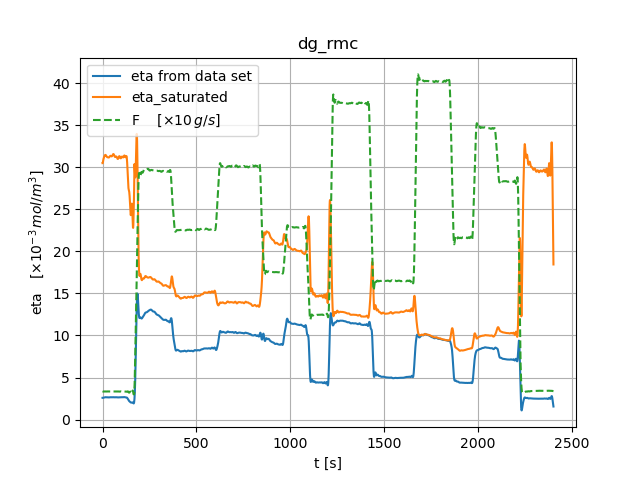
\includegraphics[width=\textwidth]{./figs/3-sysID/eta_bounds_dg_rmc.png}
    \end{minipage}
    \begin{minipage}{0.49\textwidth}
        \centering
        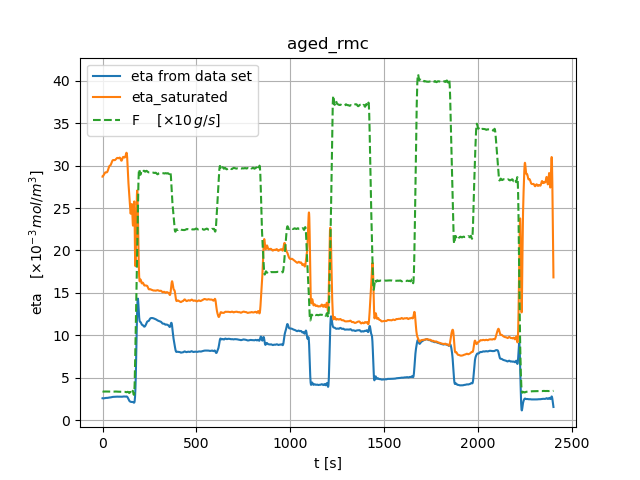
\includegraphics[width=\textwidth]{./figs/3-sysID/eta_bounds_aged_rmc.png}
    \end{minipage}
    \caption{Saturated ceiling (tight upper bound) for RMC data: degreened (left) and aged (right)}
    \label{fig::eta_bounds_rmc}
\end{figure}

\begin{figure}[!ht]
    \begin{minipage}{0.49\textwidth}
        \centering
        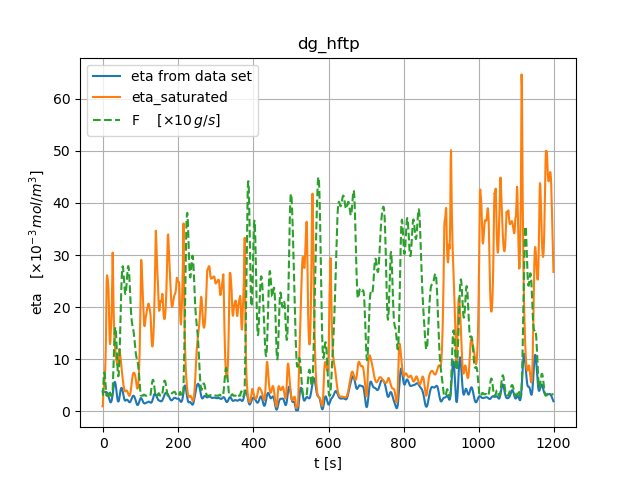
\includegraphics[width=\textwidth]{./figs/3-sysID/eta_bounds_dg_hftp.png}
    \end{minipage}
    \begin{minipage}{0.49\textwidth}
        \centering
        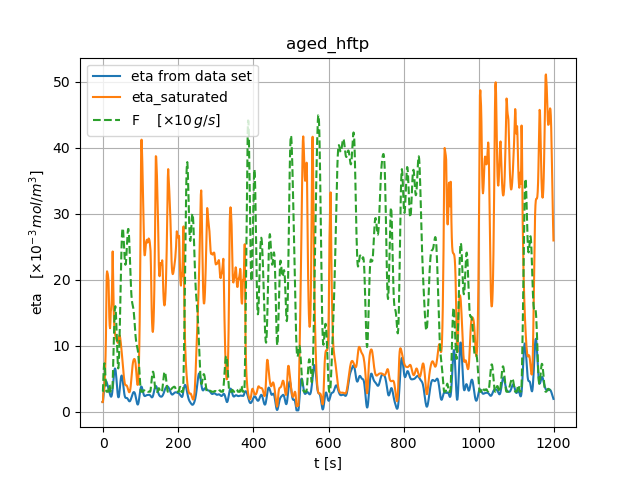
\includegraphics[width=\textwidth]{./figs/3-sysID/eta_bounds_aged_hftp.png}
    \end{minipage}
    \caption{Saturated ceiling for hot-FTP data: degreened (left) and aged (right)}
    \label{fig::eta_bounds_hftp}
\end{figure}

% --- Parameter table ---
\begin{table}[!ht]
    \centering
    \caption{$\theta_{\sat}$ estimates ($\theta_{\sat}[i]$: coefficient of $T^i$)}
    \label{tab::sat_parm_est}
    \begin{tabular}{l l r r r}
        \hline \hline
        \multicolumn{5}{c}{\textit{Degreened}} \\
        \hline
        Test & Zone & $[2]$ & $[1]$ & $[0]$ \\
        \hline
        RMC      & high & $-0.06$ & $1.43$ & $31.19$ \\
        hot-FTP  & high & $-0.49$ & $2.94$ & $40.94$ \\
        cold-FTP & high & $-0.19$ & $0.97$ & $40.69$ \\
        cold-FTP & low  & $0.26$  & $5.97$ & $45.00$ \\
        \hline
        \multicolumn{5}{c}{\textit{Aged}} \\
        \hline
        RMC      & high & $-0.07$ & $1.77$ & $27.82$ \\
        hot-FTP  & high & $-0.54$ & $3.40$ & $39.59$ \\
        cold-FTP & high & $-0.28$ & $1.82$ & $38.97$ \\
        cold-FTP & low  & $0.39$  & $8.25$ & $50.63$ \\
        \hline \hline
    \end{tabular}
\end{table}

% ===========================================================
\subsection{Segment Identification Using $\theta_{\sat}$ \label{sec::segment_id}}

With $\hat\theta_{\sat}$ estimated, the saturated model response
$\hat\eta_{\sat}(k) = \phi_{\sat}^T(k)\,\hat\theta_{\sat}$ is computed for each time step. A data point is classified
as near-saturated if the prediction error is small:
\begin{align}
    \abs{\hat\eta_{\sat}(k) - \eta(k)} \leq \varepsilon_{\sat} \implies \text{saturated operation}
    \label{eqn::sat_detect}
\end{align}
The threshold $\varepsilon_{\sat}$ is chosen from the variance of the prediction error distribution
($\varepsilon_{\sat} = 2.5\times 10^{-3}\, mol/m^{3}$ for the test-cell dataset). The saturated model response depends
only on $u_1$, $F$, and $T$ (not on the previous state or urea dosing), so it can be evaluated without simulation.

\begin{figure}[!ht]
    \centering
    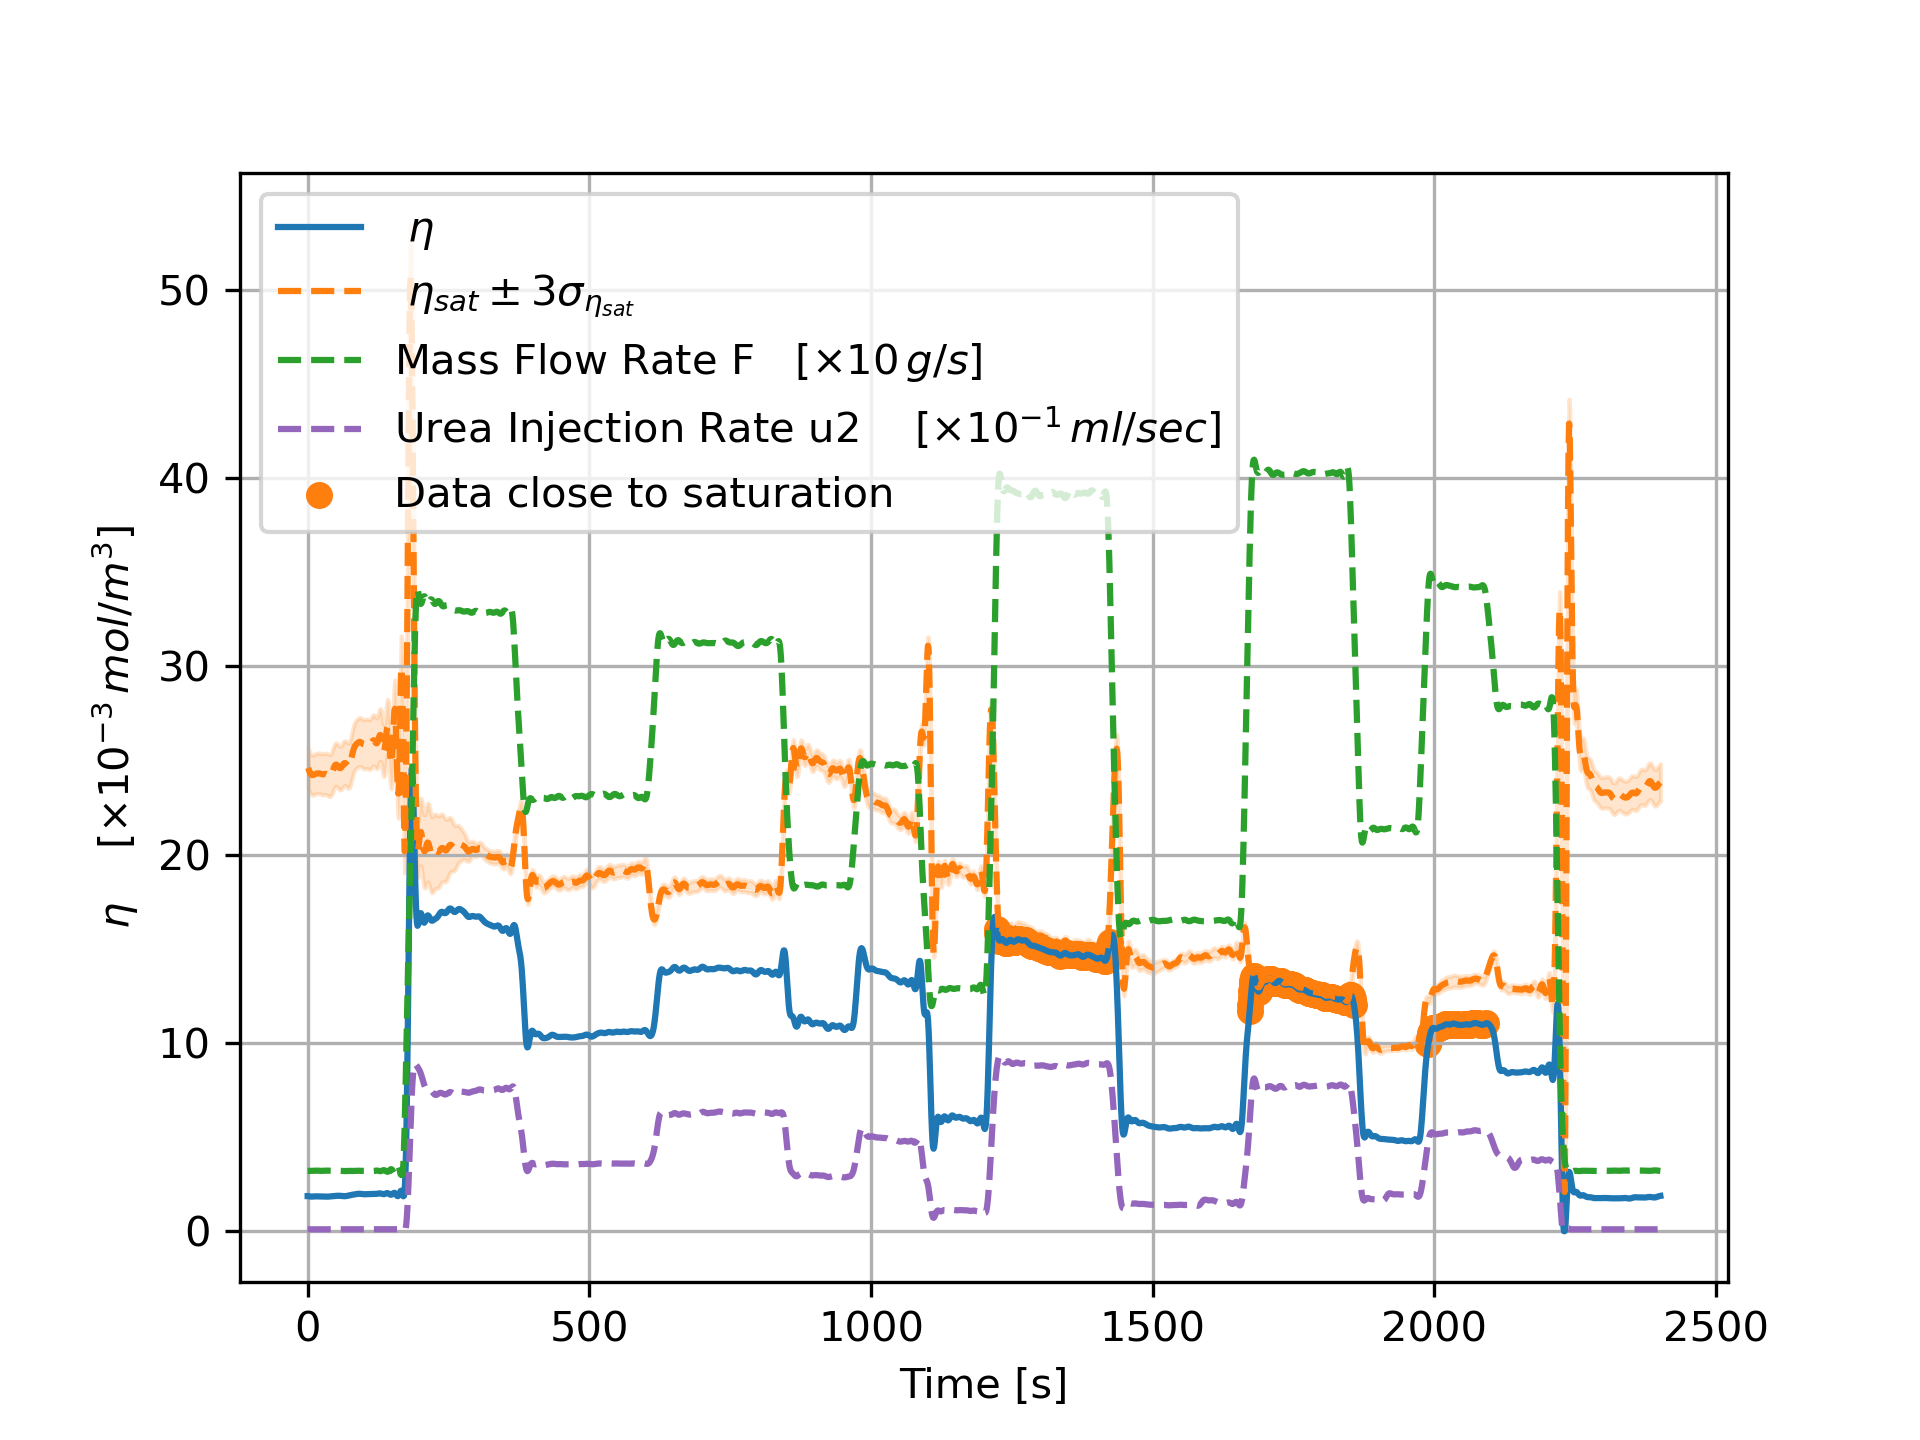
\includegraphics[width=\figWidth]{./figs/3-sysID/SatDetect_dg_rmc_1_FTIR.png}
    \caption{Catalyst mode detection for degreened RMC test-cell data}
    \label{fig::cat_mode_det}
\end{figure}

\begin{table}[!ht]
    \centering
    \caption{Data points close to catalyst saturation}
    \label{tab::sat_data_perc}
    \begin{tabular}{l r r r}
        \hline \hline
        Test & $N$ & $N_{\sat}$ (FTIR) & $N_{\sat}$ ($\nox$ sensor) \\
        \hline \hline
        DG RMC 1     & 2402 & 490 & 492 \\
        DG RMC 2     & 2402 & 493 & 494 \\
        DG RMC 3     & 2402 & 491 & 493 \\
        Aged RMC     & 2402 & 515 & 515 \\ \hline
        DG Hot FTP 1 & 634  & 186 & 194 \\
        DG Hot FTP 2 & 634  & 181 & 191 \\
        DG Hot FTP 3 & 638  & 180 & 198 \\
        Aged Hot FTP & 636  & 198 & 220 \\
        \hline \hline
    \end{tabular}
\end{table}

The unsaturated segments (the complement) are used for $\theta_{\nox}$ estimation in the next subsection.

% ===========================================================
\subsection{Unsaturated Model Parameters ($\theta_{\nox}$) \label{sec::unsat_est}}

With the saturated segments excluded, the remaining data satisfies the unsaturated
dynamics~(\ref{eqn::eta_bar_dynamics}). These data can now be used for least-squares estimation of $\theta_{\nox}$.

\subsubsection{Regression Form}

The compact form $\bar\eta_F(k{+}1) = \bar\eta_F(k) + \phi_{\nox}^T(k)\,\theta_{\nox}$~(\ref{eqn::eta_compact})
rearranges into a standard linear regression by moving $\bar\eta_F(k)$ to the left:
\begin{align}
    y_{\nox}(k) &= \phi_{\nox}^T(k)\,\theta_{\nox}
    \label{eqn::regression_form}
\end{align}
where $y_{\nox}(k) = \bar\eta_F(k{+}1) - \bar\eta_F(k)$. The regressor $\phi_{\nox}(k)$ depends only on measured
quantities and is constructed to avoid unnecessary multiplication and division of the same signals, which would amplify
noise.

$\theta_{\nox}$ is estimated by least squares on the unsaturated segments identified
in~\S\ref{sec::segment_id}. Under Gaussian model structure error, least squares is the maximum likelihood
estimate. These are the same parameters that appear in the guard
condition~(\ref{eqn::guard_condition}), so once estimated, the guard is fully determined.

\subsubsection{Estimation Results}

With both $\hat\theta_{\sat}$ and $\hat\theta_{\nox}$, the full switched model~(\ref{eqn::switched_model}) is simulated
from initial conditions and inputs ($u_1, u_2, F, T$) alone on the training data. The goodness of fit is measured by:
\begin{align}
    \%\text{fit} = 100 \times \lr{1 - \frac{\norm{Y - \hat Y}}{\norm{Y - \text{mean}(Y)}}}
\end{align}

\begin{table}[!ht]
    \centering
    \caption{Goodness of fit on training data}
    \label{tab::results}
    \begin{tabular}{l l c c}
        \hline \hline
        Age & Test & Switched model & CSTR baseline \\
        \hline \hline
        Degreened & RMC      & 71.9\% & 20.0\% \\
        Aged      & RMC      & 69.9\% & 27.7\% \\ \hline
        Degreened & hot-FTP  & 61.9\% & 7.1\%  \\
        Aged      & hot-FTP  & 63.5\% & 7.4\%  \\ \hline
        Degreened & cold-FTP & 52.9\% & 23.2\% \\
        Aged      & cold-FTP & 60.3\% & 23.2\% \\
        \hline \hline
    \end{tabular}
\end{table}

\begin{figure}[!ht]
    \begin{minipage}{0.24\textwidth}
        \centering
        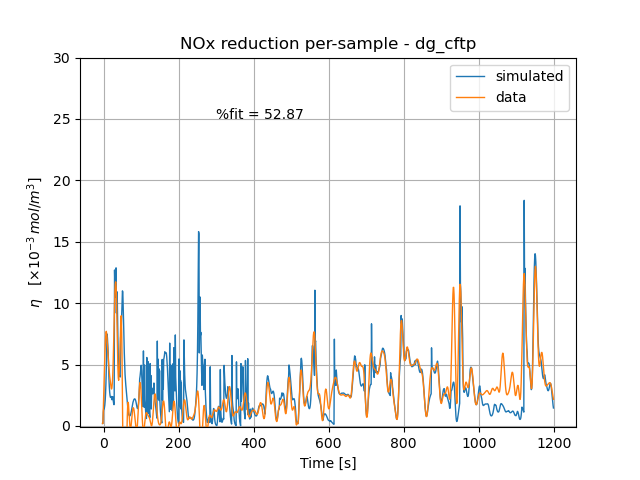
\includegraphics[width=\textwidth]{./figs/3-sysID/eta_sim_dg_cftp.png}
    \end{minipage}
    \begin{minipage}{0.24\textwidth}
        \centering
        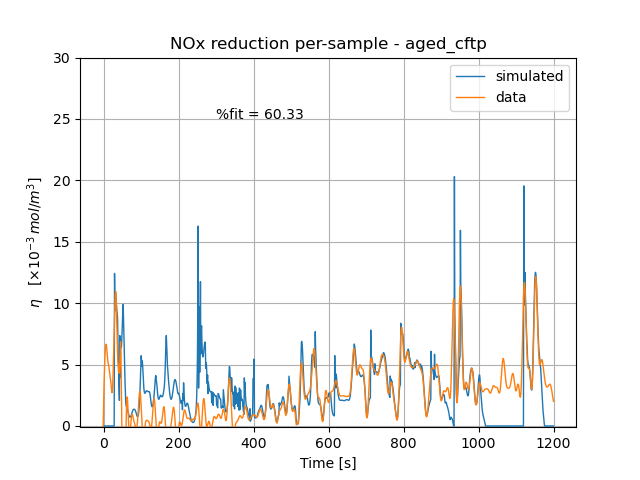
\includegraphics[width=\textwidth]{./figs/3-sysID/eta_sim_aged_cftp.png}
    \end{minipage}
    \caption{Simulation: cold-FTP}
    \label{fig::eta_sim_cftp}
\end{figure}

\begin{figure}[!ht]
    \begin{minipage}{0.24\textwidth}
        \centering
        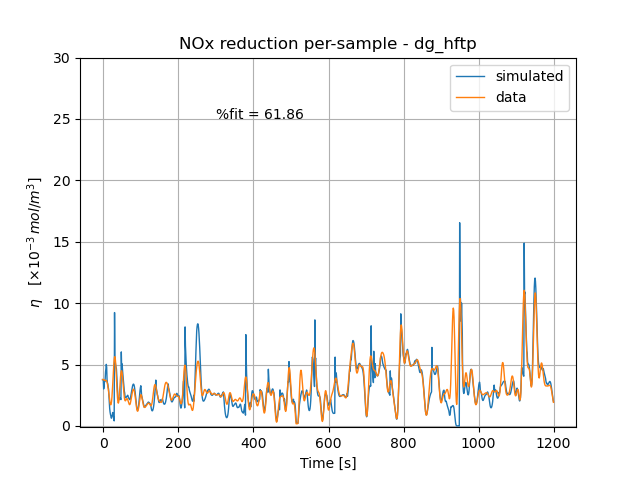
\includegraphics[width=\textwidth]{./figs/3-sysID/eta_sim_dg_hftp.png}
    \end{minipage}
    \begin{minipage}{0.24\textwidth}
        \centering
        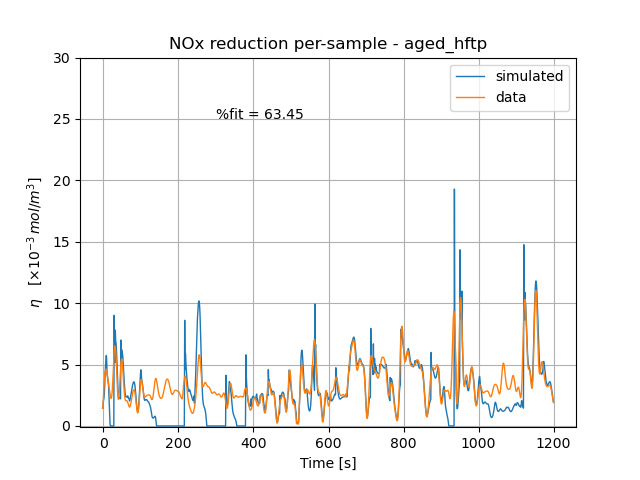
\includegraphics[width=\textwidth]{./figs/3-sysID/eta_sim_aged_hftp.png}
    \end{minipage}
    \caption{Simulation: hot-FTP}
    \label{fig::eta_sim_hftp}
\end{figure}

\begin{figure}[!ht]
    \begin{minipage}{0.24\textwidth}
        \centering
        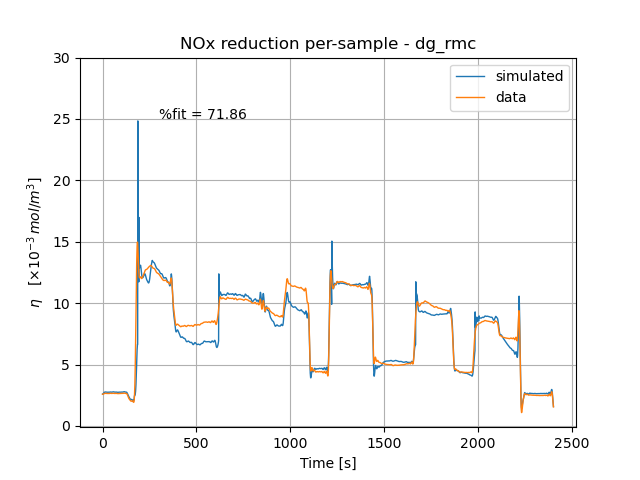
\includegraphics[width=\textwidth]{./figs/3-sysID/eta_sim_dg_rmc.png}
    \end{minipage}
    \begin{minipage}{0.24\textwidth}
        \centering
        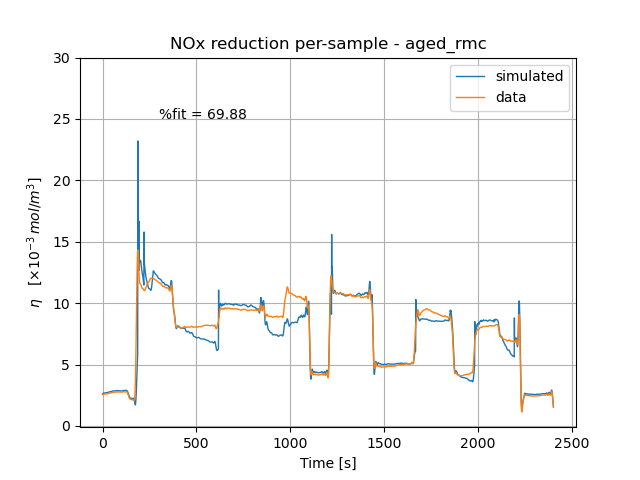
\includegraphics[width=\textwidth]{./figs/3-sysID/eta_sim_aged_rmc.png}
    \end{minipage}
    \caption{Simulation: RMC}
    \label{fig::eta_sim_rmc}
\end{figure}

% ===========================================================
\subsection{Cross-Validation \label{sec::cross_valid}}

The parameter estimates obtained from the degreened training data are applied to three additional degreened catalyst runs
(DG\_1, DG\_2, DG\_3) to test generalization.

\begin{table}[!ht]
    \centering
    \caption{Cross-validation of model parameters on additional degreened test data}
    \label{tab::cross_valid}
    \begin{tabular}{l l c}
        \hline \hline
        Age & Test & $\%$fit \\
        \hline \hline
        Degreened (train) & RMC      & 71.86 \\
        DG\_1             & RMC      & 67.12 \\
        DG\_2             & RMC      & 54.71 \\
        DG\_3             & RMC      & 67.01 \\ \hline
        Degreened (train) & hot-FTP  & 61.86 \\
        DG\_1             & hot-FTP  & 54.87 \\
        DG\_2             & hot-FTP  & 59.44 \\
        DG\_3             & hot-FTP  & 50.17 \\ \hline
        Degreened (train) & cold-FTP & 52.87 \\
        DG\_1             & cold-FTP & 39.41 \\
        DG\_2             & cold-FTP & 41.52 \\
        DG\_3             & cold-FTP & 42.17 \\
        \hline \hline
    \end{tabular}
\end{table}

The model generalizes across runs, with cross-validation $\%$fit values within $10$--$15$ percentage points of the
training fit.

% ===========================================================
